\section{Results} \label{sec:results}
\subsection{Input generation}
We generate our piecewise DOG quad mesh based on an input SVG file specifying the crease pattern. The input file contains polylines for creases and boundary loops. We use CGAL's arrangement model \cite{cgal} to compute the decomposition induced by the polylines and place an orthogonal grid of a given mesh resolution on top of the entire model, where quads that appear on multiple components are duplicated (see \figref{fig:piecewise_dog_from_crease}). We snap nearby intersections or starting points of non-closed polylines to one another. To get a correct arrangement topology, every curve intersection with other curves or boundary loops needs to be on the orthogonal grid line, i.e. on an edge or a vertex, and we snap their x and y coordinates to prevent the grid from having very thin squares. For rendering purposes, we keep another mesh where the extraneous parts of the duplicated faces are culled.
\subsection{Editing system}
\MiR{Important: Enforcing the folding constraint automatically choose M/V assignment (show figure). Also write it down in figures.}
\begin{figure} [h]
	\centering
	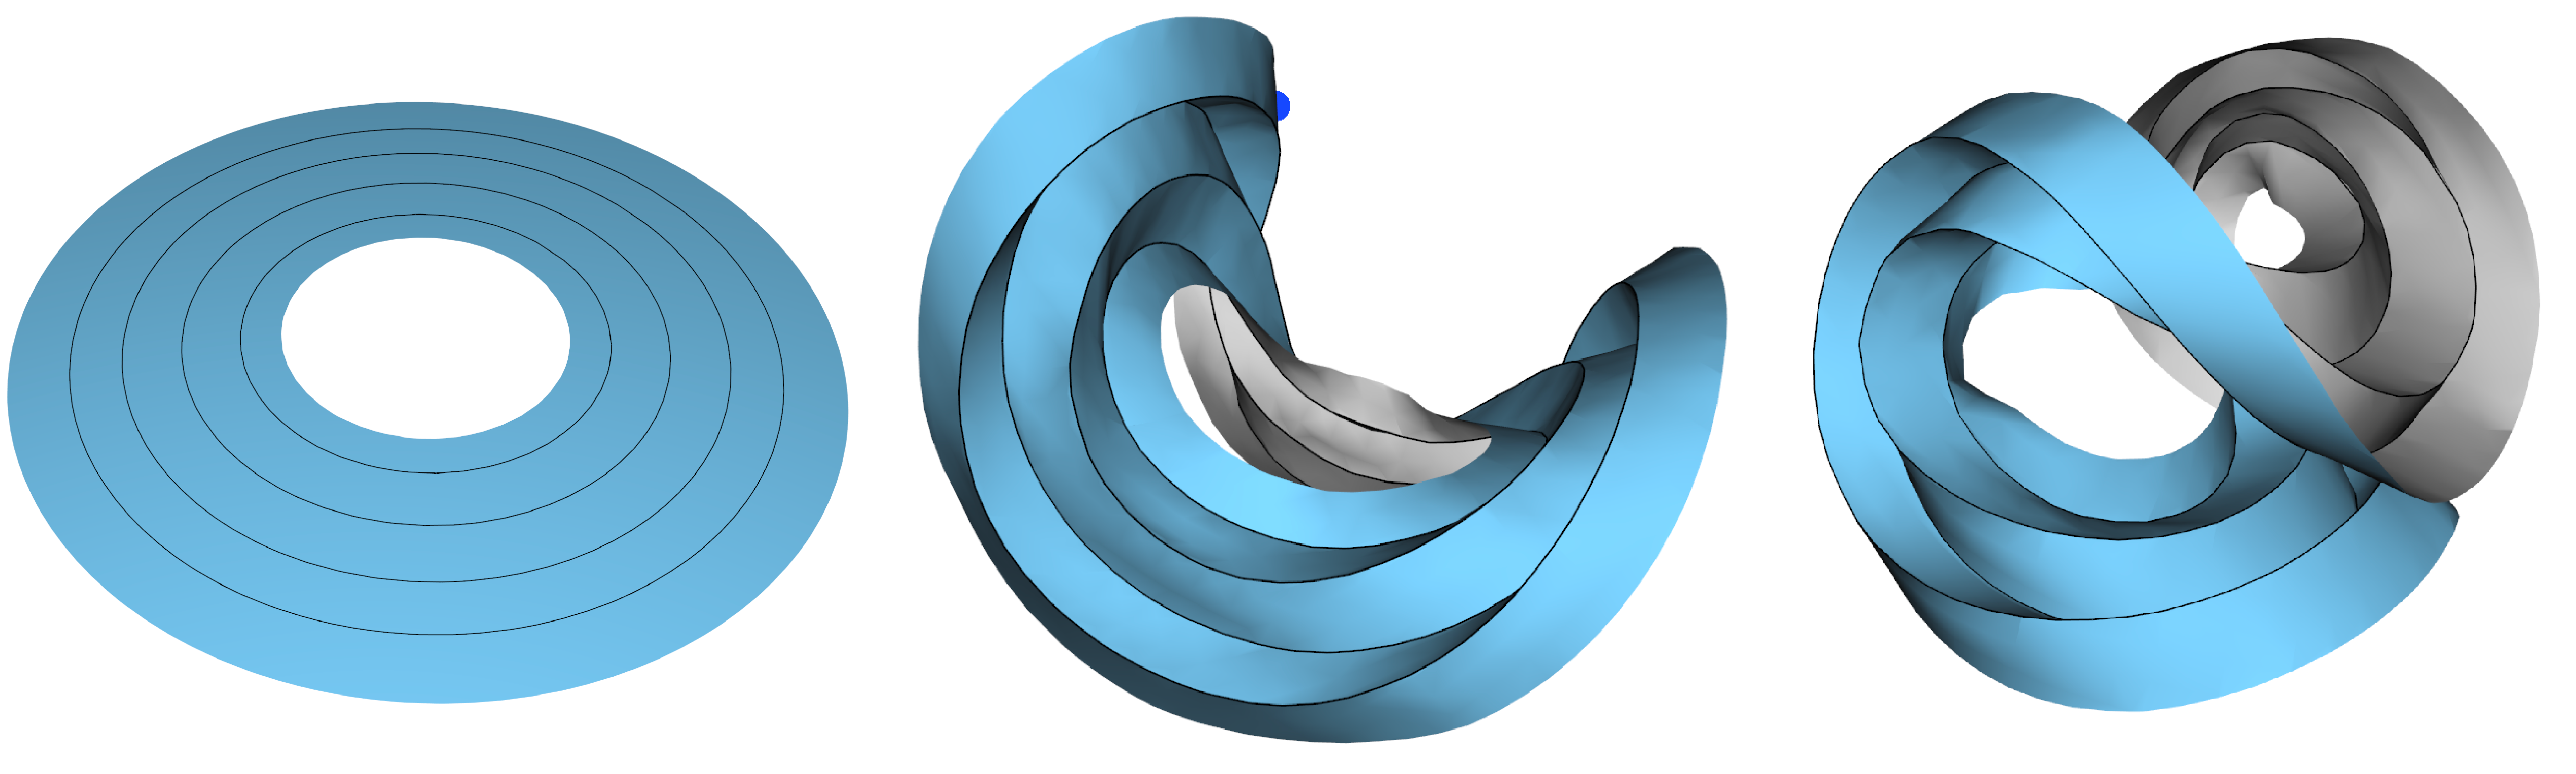
\includegraphics[width=\linewidth]{figures/annulus}
	\caption{\MiR{probably a temporary figure} }
	\label{fig:annulus}
\end{figure}
\subsection{Symmetry}
\subsection{Moving creases}